\documentclass[Hovedrapport.tex]{subfiles}
    \begin{document}
%--------------------------------------------------------------------
%\frontmatter
%\subfile{Rapporten/0000_Forside_bilag.tex}
%\clearpage                     % T.o.C. begyndes på ny side
%\newpage                       % Resten af siden for T.o.C. tømmes
\setcounter{section}{0} 	    % Sidetals nr. nulstilles
%\mainmatter                    % Lang forklaring...Bare ignorér der!
%--------------------------------------------------------------------
\chapter{Bilag}       
\label{chap:blg}
\vspace{-30pt}
\counterwithout{section}{chapter}
\renewcommand{\thesection}{B\arabic{section}}
%-------------------------------------------------------------------------------
%---------------------- ERFARINGSTAL FOR VARMEOVERGANGSTAL ---------------------
%-------------------------------------------------------------------------------
\newpage
\section{Erfaringstal}
    \label{sec:bil_erfaringstal_U}
Herunder fremgår erfaringstal for varmegennemgangstallet, U (Powerpoint lektion 7, Termodynamikundervisning):
\begin{figure}[H]
    \centering
    \includegraphics[width=1.0\textwidth]{Billeder/bil_erfaringstal_U.PNG}
    \caption{\textit{Erfaringsværdier for varmeovergangstallet}.}
    \label{fig:bil_erfaringstal_U}
\end{figure}

%-------------------------------------------------------------------------------
%------------------------------ DATABLAD FOR KOMPRESSOR ------------------------
%-------------------------------------------------------------------------------
\newpage
\section{Datablad for BD350GH kompressor fra Danfoss}
\label{sec:bil_kom}
Dette bilag omhandler databladet for kompressoren. De data er blandt andet brugt til at beregne den volumetriske- og isentrope virkningsgrad. Databladet er også brugt til programmering af kompressoren.\\ 
\begin{minipage}{1.0\textwidth}
\includepdf[pages={1}, scale=.7, pagecommand=\pagestyle{fancy}, offset=0 1cm]{Billeder/bd350gh.pdf}
\end{minipage}

\includepdf[pages={2}, scale=.8,pagecommand={\pagestyle{fancy}}, offset=0 1cm]{Billeder/bd350gh.pdf}


%-------------------------------------------------------------------------------
%------------------------------ KOMPRESSOR COOLPACK ----------------------------
%-------------------------------------------------------------------------------
\newpage
\section{BD350GH 24 V kompressor Coolselector}
    \label{sec:bil_kompressor_coolpack}
I Nedenstående bilag ses databladet for kompressoren BD350GH 24 V fra Danfoss. Databladet er fundet i coolselector, hvori kompressoren også er valgt på baggrund af dens forslag.
\begin{minipage}{1.0\textwidth}
\includepdf[pages={1}, scale=.7, pagecommand={\pagestyle{fancy}}, offset=0 -3cm]{Billeder/BD350GH_24V_Coolselector.pdf}
\end{minipage}


%-------------------------------------------------------------------------------
%------------------------- DATABLAD FOR EKSPANSIONSVENTIL ----------------------
%-------------------------------------------------------------------------------
\newpage
\section{Datablad for ekspansinsventil T2 fra Danfoss}{\label{sec:bil_ventil}}

I dette billag ses hvilket kriterier ekspansionsventilen er udvalgt under. Fra værkstedet var der en T2 ekspansionsventil tilrådighed. Denne er med udskiftelig dyse. Ud fra coolselecotr er dysen X0 valgt, da denne giver de ønskede massestrømme. 
%----------------------------------- SIDE 1 -------------------------------------
\begin{minipage}{1.0\textwidth}
\includepdf[pages={1}, scale=.8, pagecommand={\pagestyle{fancy}}, offset=0 -1cm]{Billeder/Ekspansionsventil_Danfoss_billag.pdf}
\end{minipage}
%----------------------------------- SIDE 2 -------------------------------------
\includepdf[pages={2}, scale=.85, pagecommand={\pagestyle{fancy}}, offset=0 0cm]{Billeder/Ekspansionsventil_Danfoss_billag.pdf}


%-------------------------------------------------------------------------------
%--------------------------- Danfoss datablad dyser ----------------------------
%-------------------------------------------------------------------------------
\newpage
\section{Dysevalg til Danfoss T2 ekspansionsventil}
    \label{sec:bil_Danfos_dysevalg}
I Nedenstående bilag ses databladet valg af dyse størrelse til T2 ekspansionsventil. Dette datablad er brugt til at kontrollere valget af dyse til T2 ekspansionsventilen i Coolselector.
%----------------------------------- SIDE 1 -------------------------------------
\begin{minipage}{1.0\textwidth}
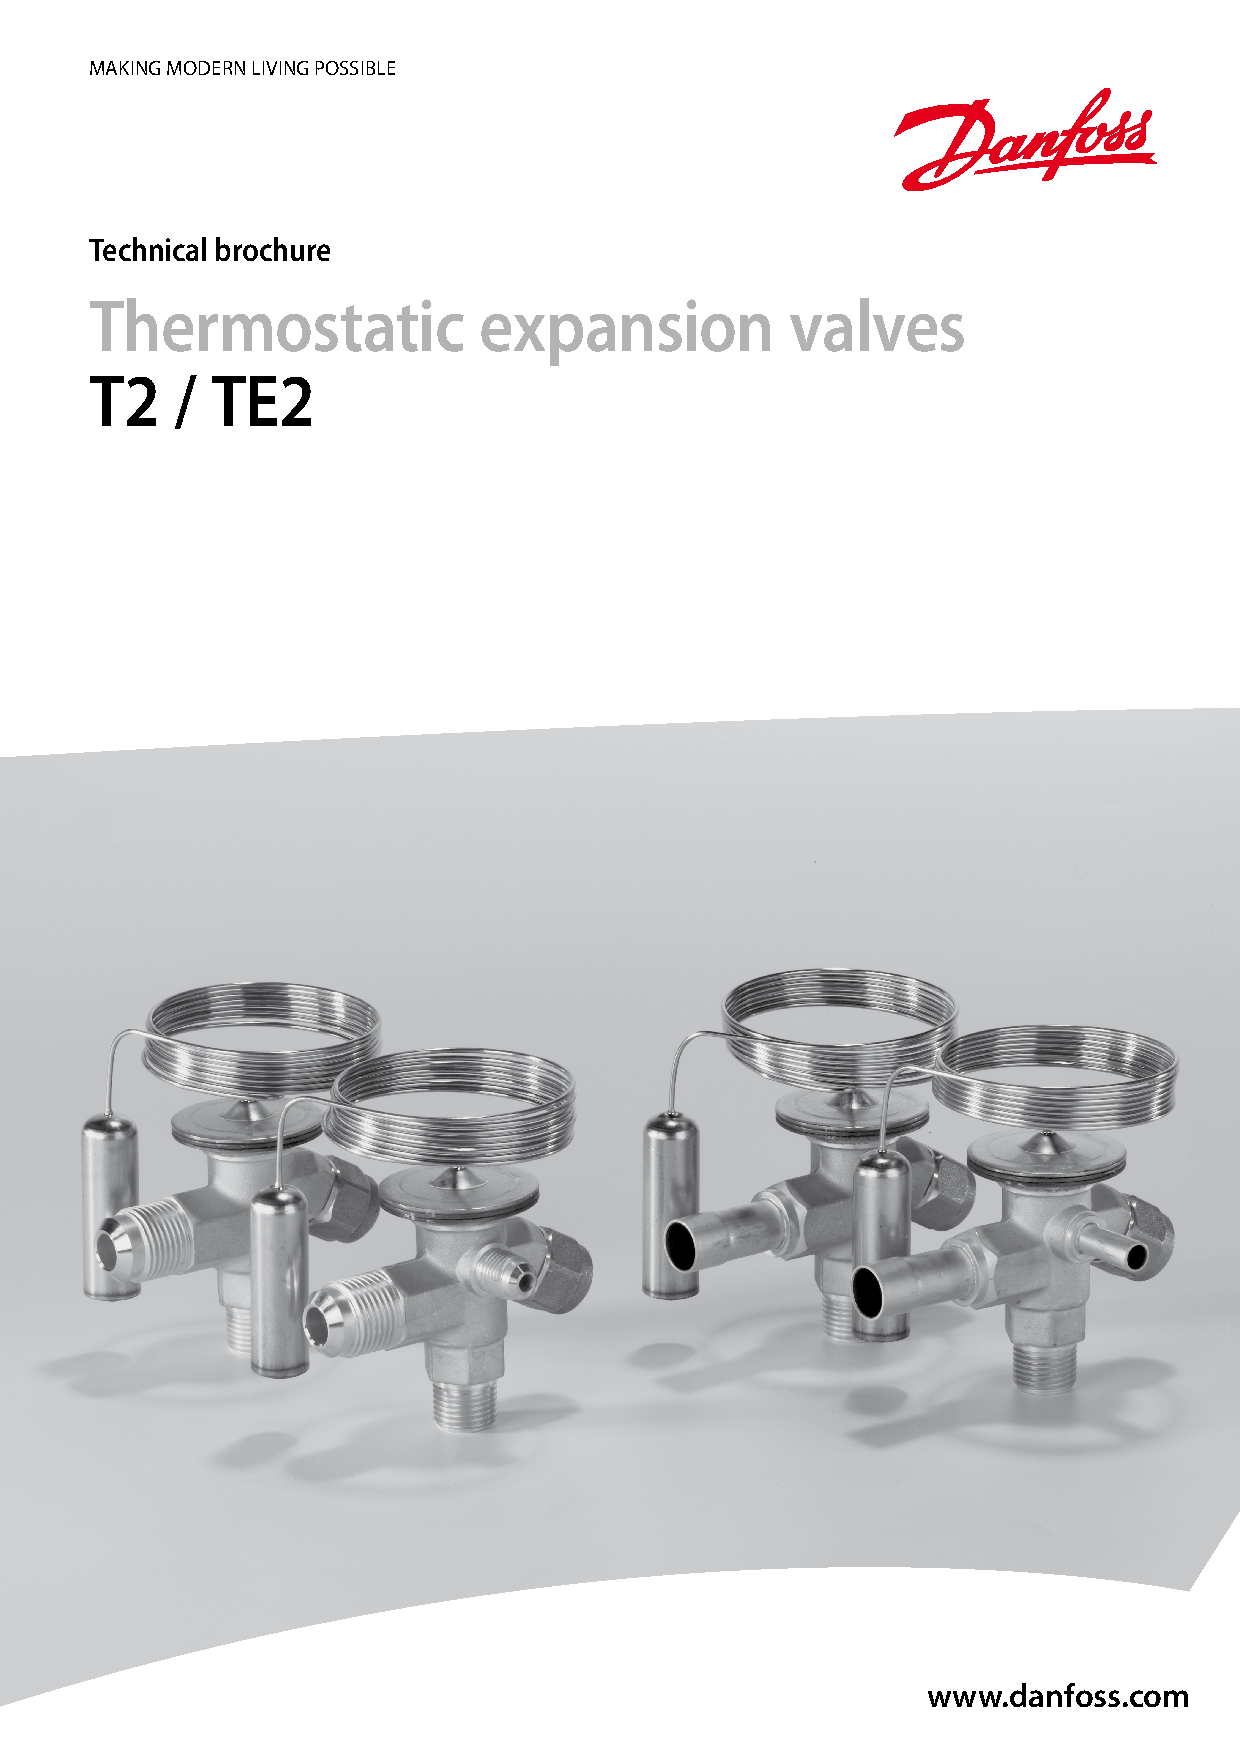
\includepdf[pages={1}, scale=.7, pagecommand={\pagestyle{fancy}}, offset=0 0cm]{Billeder/Ekspansionsventil_Danfoss_Datablad.pdf}
\end{minipage}
\newpage

%----------------------------------- SIDE 2 -------------------------------------
\includepdf[pages={2}, scale=.85, pagecommand={\pagestyle{fancy}}, offset=0 0cm]{Billeder/Ekspansionsventil_Danfoss_Datablad.pdf}

%----------------------------------- SIDE 3 -------------------------------------
\includepdf[pages={3}, scale=.85, pagecommand={\pagestyle{fancy}}, offset=0 0cm]{Billeder/Ekspansionsventil_Danfoss_Datablad.pdf}

%----------------------------------- SIDE 8 -------------------------------------
\includepdf[pages={8}, scale=.85, pagecommand={\pagestyle{fancy}}, offset=0 0cm]{Billeder/Ekspansionsventil_Danfoss_Datablad.pdf}






%-------------------------------------------------------------------------------
%------------------------ DATABLAD FOR AKS32 TRYKTRANSMITTER -------------------
%-------------------------------------------------------------------------------
\newpage
\section{Datablad for Danfoss AKS32 tryktransmitter}
\label{sec:bil_tryk}
I dette bilag findes databladet for AKS32 tryktransmitter, som er brugt til at måle fordampnings- og kondenserings tryk i køleanlægget. 

\begin{minipage}{1.0\textwidth}
\includepdf[pages={1}, scale=.7, pagecommand={\pagestyle{fancy}}, offset=0 0cm]{Billeder/bil_aks32_datablad.pdf}
\end{minipage}

\includepdf[pages={2,5}, scale=.8,pagecommand={\pagestyle{fancy}}, offset=0 0cm]{Billeder/bil_aks32_datablad.pdf}




%--------------------------
%----------------------------------------------------
\clearpage
%-------------------------------------------------------------------------------
\end{document}
